% -----------------------------------------------------------------
% Document class: Article
\documentclass[ a4paper, twoside, 11pt]{article}
\usepackage{../../macros-general}
\usepackage{../../macros-article}
% Number of the handout, quiz, exam, etc.
\newcommand{\numero}{02}
\setcounter{numero}{\numero}
\graphicspath{{./figures/}}

% -----------------------------------------------------------------
\begin{document}
\allowdisplaybreaks

% Indices
\newcommand{\iava}{$i$\tsup{ava} }
\newcommand{\iavo}{$i$\tsup{avo} }
\newcommand{\java}{$j$\tsup{ava} }
\newcommand{\javo}{$j$\tsup{avo} }
\newcommand{\kava}{$k$\tsup{ava} }
\newcommand{\kavo}{$k$\tsup{avo} }
\newcommand{\tava}{$t$\tsup{ava} }
\newcommand{\tavo}{$t$\tsup{avo} }
\newcommand{\tmava}{$(t-1)$\tsup{ava} }
\newcommand{\tmavo}{$(t-1)$\tsup{avo} }
\newcommand{\tMava}{$(t+1)$\tsup{ava} }
\newcommand{\tMavo}{$(t+1)$\tsup{avo} }

\begin{center}
\Large Modelos Estoc\'asticos (INDG-1008): Examen \numero \\[2ex]
\small \textbf{Semestre:} 2017-2018 T\'ermino II \qquad
\textbf{Instructor:} Luis I. Reyes Castro
\end{center}
\fullskip

% -----------------------------------------------------------------
\begin{problem}
La sala de emergencias de un peque\~no hospital cuenta con dos doctores, quienes cuentan con sus propios consultorios y quir\'ofanos, adem\'as de cuatro camillas de espera. \linebreak Los pacientes arriban a una tasa promedio de 1.8 por hora y son atendidos por orden de arribo. \linebreak Todo paciente que arriba cuando todas las camillas de espera est\'an ocupadas es enviado directamente a otro hospital. Los tiempos que necesitan los doctores para atender a los pacientes est\'an exponencialmente distribuidos, con un promedio de 40 minutos. Despu\'es de ser atendido, cada paciente es referido a otra \'area de especialidad del hospital o dado de alta. 

Con esto en mente, complete las siguientes actividades: 
\begin{enumerate}[label=\textbf{\alph*)}]
\item \textbf{1 Punto:} Indique, utilizando notaci\'on de Kendall, qu\'e tipo de sistema de cola es este, y bosqueje la Cadena de Markov en Tiempo Continuo correspondiente. \\[1ex]
\emph{Soluci\'on:} Este sistema de colas es del tipo M/M/2/6, y la cadena correspondiente se muestra en la siguiente fotograf\'ia. 
\begin{figure}[htb]
\centering
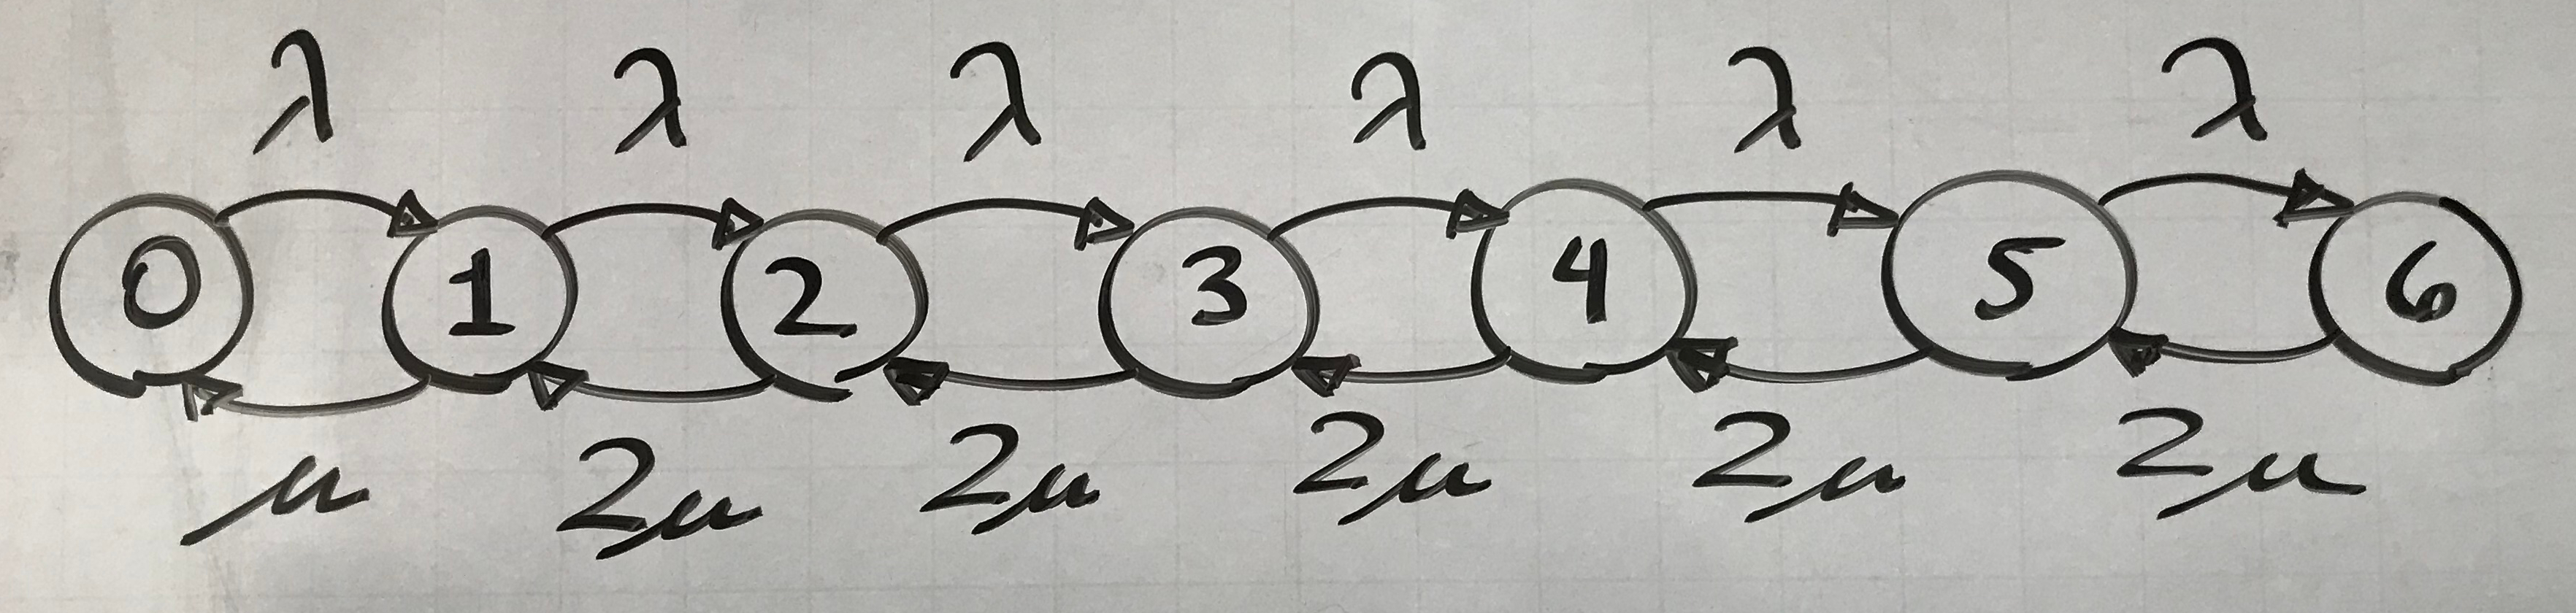
\includegraphics[width=0.66\textwidth]{Problema-1A.jpg}
\end{figure}

\item \textbf{4 Puntos:} Encuentre la distribuci\'on estacionaria del sistema. \\[1ex]
\emph{Soluci\'on:} Dado que la tasa de arribo es $\lambda = 1.8$ pacientes por hora y la tasa de servicio por doctor es de $\mu = 1.5$ pacientes por hora, si definimos $\rho \define \lambda / 2 \mu = 0.6$ como de costumbre las ecuaciones de balance son: 
\begin{align*}
& E_0 \; \colon \; \lambda \, \pi_0 \; = \; \mu \, \pi_1
\quad \Longrightarrow \quad
\pi_1 \; = \; 2 \, \rho \, \pi_0 \\
& E_1 \; \colon \; (\lambda + \mu) \, \pi_1
\; = \; \lambda \, \pi_0 + 2 \, \mu \, \pi_2
\quad \Longrightarrow \quad
\pi_2 \; = \; 2 \, \rho^2 \, \pi_0 \\
& E_2 \; \colon \; (\lambda + 2 \mu) \, \pi_2
\; = \; \lambda \, \pi_1 + 2 \, \mu \, \pi_3
\quad \Longrightarrow \quad
\pi_3 \; = \; 2 \, \rho^3 \, \pi_0 \\
& \cdots \\
& E_k \; \colon \; (\lambda + 2\mu) \, \pi_{k} \; = \; \lambda \, \pi_{k-1} + 2 \, \mu \, \pi_{k+1} \quad \Longrightarrow \quad
\pi_{k+1} \; = \; 2 \, \rho^{k+1} \, \pi_0 \\
& \cdots
\end{align*}
Ahora normalizamos para hallar la probabilidad del estado cero: 
\[
\pi_0 + 
2 \, \pi_0 \, \sum_{k=1}^6 \rho^k \; = \; 1 \quad \Longrightarrow \quad
\pi_0 \; = \; \left( 1 + 2 \, \sum_{k=1}^6 \rho^k \right)^{-1}
\; = \; 0.259
\]
Consecuentemente, la distribuci\'on estacionaria del sistema es: 
\begin{table}[H]
\centering
\begin{tabular}{|c|c|}
\hline
\textbf{Estado} $\boldsymbol{i}$ & $\boldsymbol{\pi_i}$ \\ \hline
0 & 0.259 \\ \hline
1 & 0.311 \\ \hline
2 & 0.186 \\ \hline
3 & 0.112 \\ \hline
4 & 0.067 \\ \hline
5 & 0.040 \\ \hline
6 & 0.024 \\ \hline
\end{tabular}
\end{table}

\item \textbf{2 Puntos:} Calcule el n\'umero esperado de pacientes en cola, junto con el tiempo esperado de espera en cola. \\[1ex]
\emph{Soluci\'on:} Puesto que este sistema cuenta con dos servidores, el n\'umero esperado de clientes en cola es: 
\[
\overline{L_q} \; = \;
\Exp[ \, \max \, \{ \, 0, \, X_t-2 \, \} \, ] \; = \;
\sum_{k=2}^6 (k-2) \, \pi_k \; = \; 0.464
\]
Ahora calculamos el tiempo esperado de espera en cola utilizando la Ley de Little: 
\[
\overline{L_q} \; = \; \lambda \, \overline{W_q}
\quad \Longrightarrow \quad
\overline{W_q} \; = \; \frac{\overline{L_q}}{\lambda} \; = \; 0.258 \; \text{horas} \; \equiv \; 15.47 \; \text{minutos}
\]

\item \textbf{1 Punto:} En el enunciado del problema original, suponga que hubiere cuatro doctores en vez de dos, cada uno con su propio consultorio y quir\'ofano. Indique, utilizando notaci\'on de Kendall, qu\'e tipo de sistema de cola es este, y bosqueje la Cadena de Markov en Tiempo Continuo correspondiente. \\[1ex]
\emph{Soluci\'on:} Este sistema de colas es del tipo M/M/4/8, y la cadena correspondiente se muestra en la siguiente fotograf\'ia. 
\begin{figure}[htb]
\centering
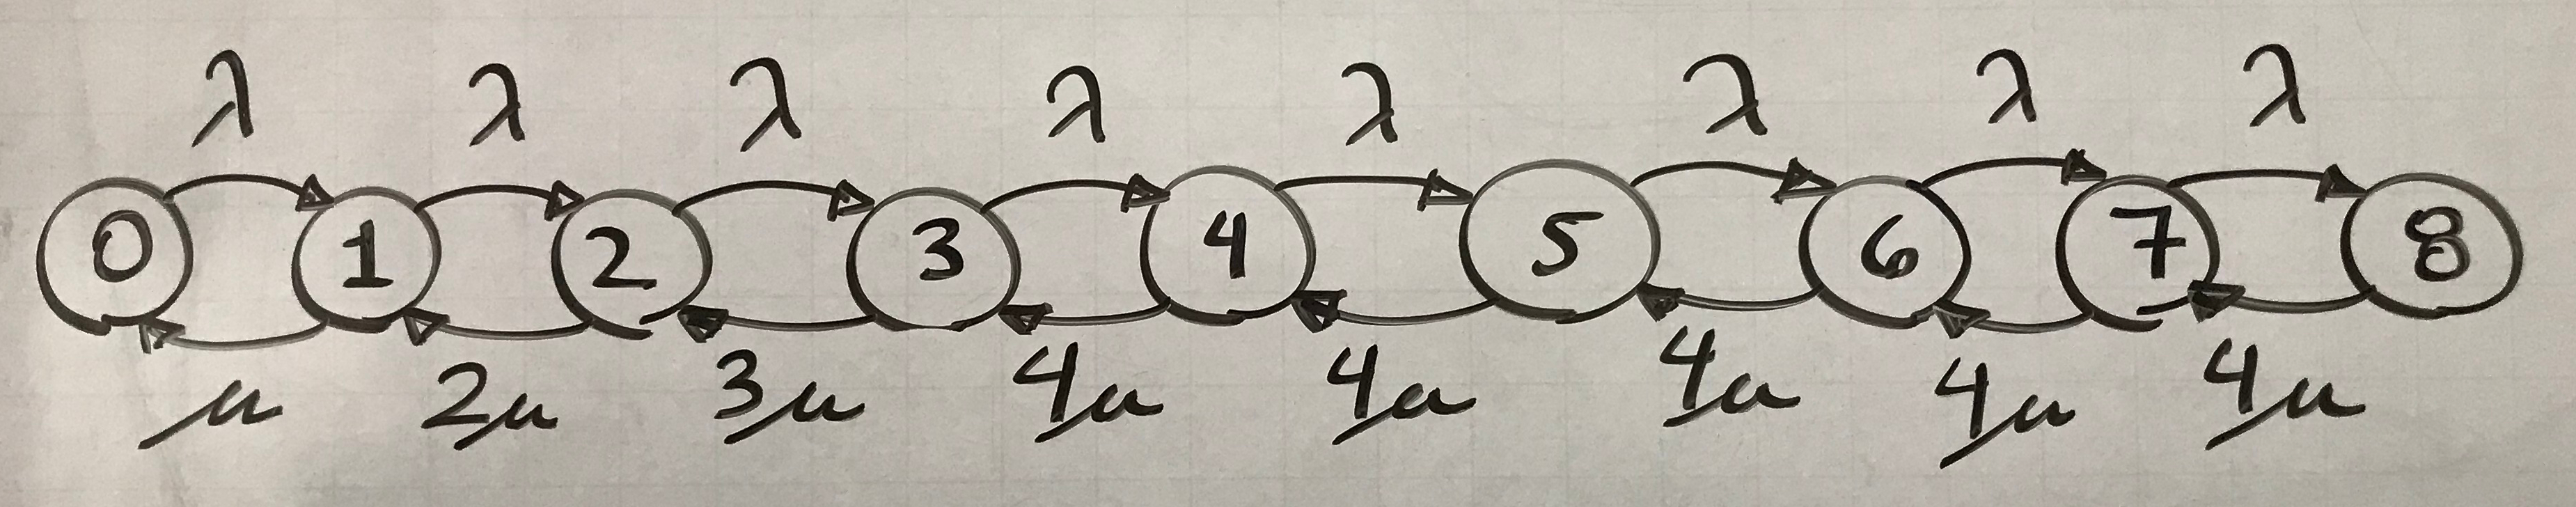
\includegraphics[width=0.76\textwidth]{Problema-1C.jpg}
\end{figure}

\item \textbf{1 Punto:} En el enunciado del problema original, suponga que hubiere cinco camillas de espera en vez de cuatro. Indique, utilizando notaci\'on de Kendall, qu\'e tipo de sistema de cola es este, y bosqueje la Cadena de Markov en Tiempo Continuo correspondiente. \\[1ex]
\emph{Soluci\'on:} Este sistema de colas es del tipo M/M/2/7, y la cadena correspondiente se muestra en la siguiente fotograf\'ia. 
\begin{figure}[htb]
\centering
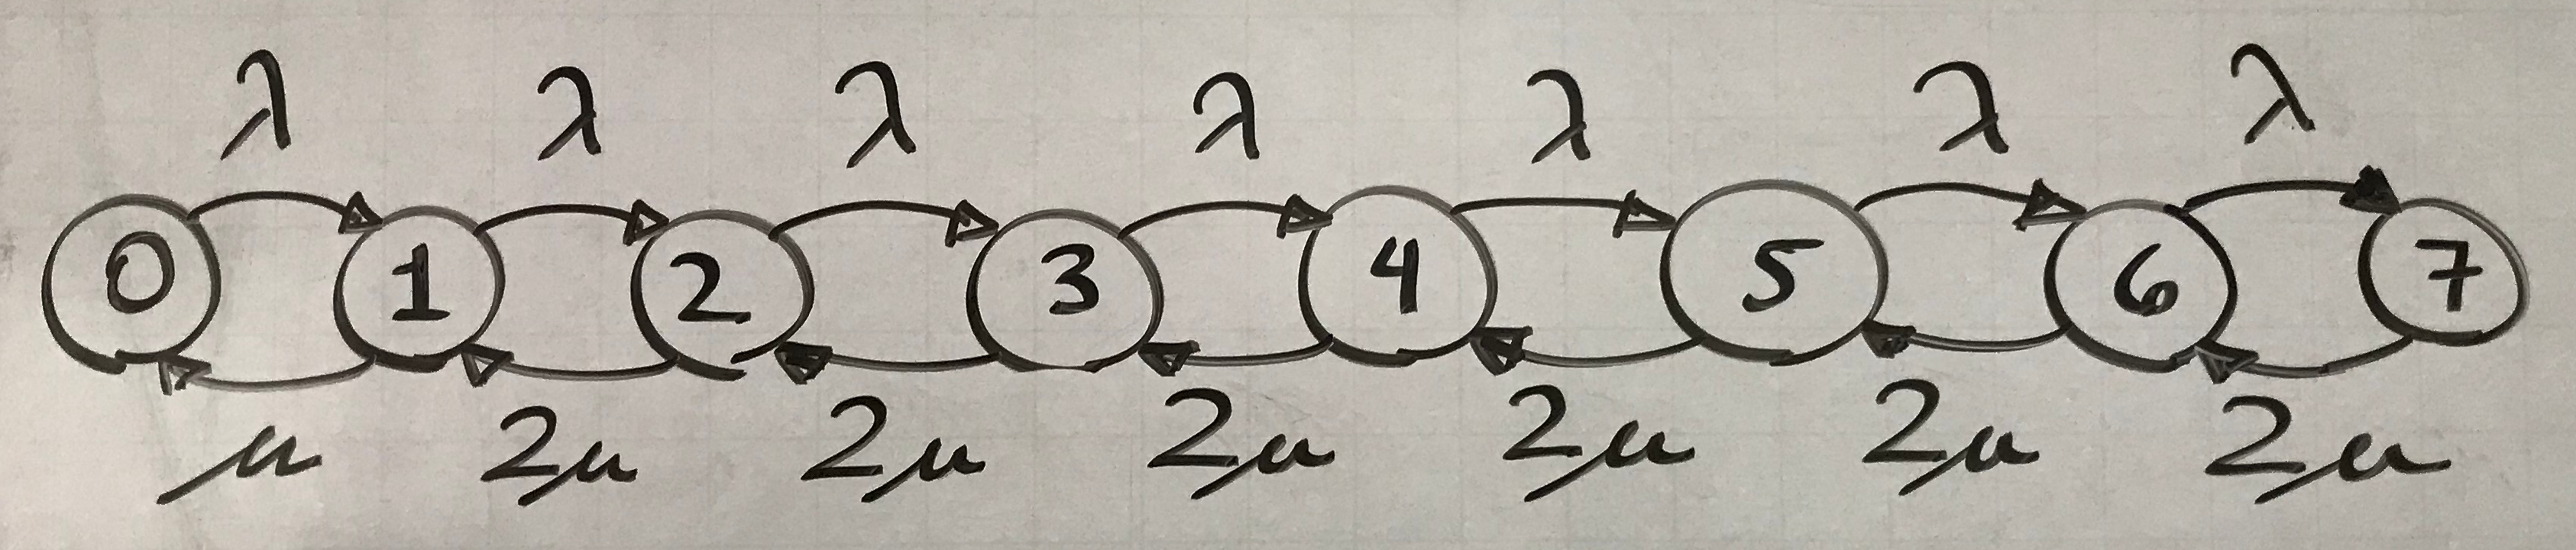
\includegraphics[width=0.66\textwidth]{Problema-1D.jpg}
\end{figure}

\end{enumerate}
\QED

\end{problem}
\fullskip

% -----------------------------------------------------------------
\begin{problem}
\textbf{[8 Puntos]} El Prof. Reyes entren\'o una red neuronal convolucional para detectar barcos en im\'agenes satelitales, la cual (por falta de imaginaci\'on) bautiz\'o como \emph{BarcoNet}. Este modelo fue entrenado para clasificar im\'agenes de acuerdo a \textit{(i)} la ausencia de barcos, \linebreak \textit{(ii)} la presencia de barcos de turismo, \textit{(iii)} la presencia de barcos de pesca o \textit{(iv)} la presencia de barcos de guerra. El entrenamiento se llev\'o a cabo utilizando un juego de im\'agnes artificialmente generadas, donde cada una de las clases anteriormente descritas ocurr\'ia con la misma probabilidad. Como resultado del entrenamiento, se obtuvo un modelo de clasificaci\'on con la siguiente matriz de confusi\'on: 
\begin{table}[H]
\centering
\begin{tabular}{c|c|c|c|c|}
\cline{2-5}
 & \multicolumn{4}{c|}{\textbf{Clase Predecida} $\boldsymbol{Y}$} \\ \hline
\multicolumn{1}{|c|}{\textbf{Clase Real} $\boldsymbol{X}$} & \textbf{Nada} & \textbf{B-Turismo} & \textbf{B-Pesca} & \textbf{B-Guerra} \\ \hline
\multicolumn{1}{|c|}{\textbf{Nada}} & 0.96 & 0.02 & 0.01 & 0.01 \\ \hline
\multicolumn{1}{|c|}{\textbf{B-Turismo}} & 0.01 & 0.88 & 0.08 & 0.03 \\ \hline
\multicolumn{1}{|c|}{\textbf{B-Pesca}} & 0.03 & 0.07 & 0.85 & 0.05 \\ \hline
\multicolumn{1}{|c|}{\textbf{B-Guerra}} & 0.02 & 0.03 & 0.04 & 0.91 \\ \hline
\end{tabular}
\end{table}

Ahora, suponga que \emph{BarcoNet} es probada por la Marina en las Gal\'apagos. Para esto, se llev\'o a cabo un muestreo de im\'agenes satelitales del archipi\'elago, donde se encontr\'o que cada una de las clases aparece con la frencuencia mostrada en la siguiente tabla. 

\begin{table}[H]
\centering
\begin{tabular}{|c|c|c|c|c|}
\hline
\textbf{Clase Real $\boldsymbol{X}$} & \textbf{Nada} & \textbf{B-Turismo} & \textbf{B-Pesca} & \textbf{B-Guerra} \\ \hline
\textbf{Frecuencia} & 0.82 & 0.10 & 0.06 & 0.02 \\ \hline
\end{tabular}
\end{table}

Con todo esto en mente, calcule la distribuci\'on posterior predictiva de \emph{BarcoNet} con respecto a la distribuci\'on de im\'agenes de las Gal\'apagos. 

\emph{Soluci\'on:} Primero recordamos c\'omo se calcula la distribuci\'on posterior: 
\[
\forall \, y \; \colon \;
\Pr( \, Y = y \, ) \; = \;
\sum_{\text{clases }x}
\Pr( \, X = x \, ) \, \Pr( \, Y = y \mid X = x \, )
\]
Entonces la distribuci\'on posterior es: 
\begin{table}[H]
\centering
\begin{tabular}{|c|c|c|c|c|}
\hline
\textbf{Clase Predecida $\boldsymbol{Y}$} & \textbf{Nada} & \textbf{B-Turismo} & \textbf{B-Pesca} & \textbf{B-Guerra} \\ \hline
\textbf{Frecuencia} & 0.7904 & 0.1092 & 0.0680 & 0.0324 \\ \hline
\end{tabular}
\end{table}
Luego recordamos c\'omo se calcula la distribuci\'on posterior predictiva: 
\[
\forall \, x, \, \forall \, y \; \colon \;
\Pr( \, X = x \mid Y = y \, ) \; = \;
\frac{ \Pr( \, X = x \, ) \, \Pr( \, Y=y \mid X=x \, )}{ \Pr( \, Y = y \, )}
\]
Finalmente, la distribuci\'on posterior predictiva es: 
\begin{table}[H]
\centering
\begin{tabular}{c|c|c|c|c|}
\cline{2-5}
 & \multicolumn{4}{c|}{\textbf{Clase Real} $\boldsymbol{X}$} \\ \hline
\multicolumn{1}{|c|}{\textbf{Clase Predecida} $\boldsymbol{Y}$} & \textbf{Nada} & \textbf{B-Turismo} & \textbf{B-Pesca} & \textbf{B-Guerra} \\ \hline
\multicolumn{1}{|c|}{\textbf{Nada}} & 0.9960 & 0.0013 & 0.0023 & 0.0005 \\ \hline
\multicolumn{1}{|c|}{\textbf{B-Turismo}} & 0.1502 & 0.8059 & 0.0385 & 0.0055 \\ \hline
\multicolumn{1}{|c|}{\textbf{B-Pesca}} & 0.1206 & 0.1176 & 0.7500 & 0.0118 \\ \hline
\multicolumn{1}{|c|}{\textbf{B-Guerra}} & 0.2531 & 0.0926 & 0.0926 & 0.5617 \\ \hline
\end{tabular}
\end{table}
\QED

\end{problem}
\fullskip

% -----------------------------------------------------------------
\begin{problem}
\textbf{[6 Puntos]} Un acaudalado inversionista tiene una empresa que se dedica a identificar \emph{start-ups} prometedoras. De las empresas que \'el usualmente eval\'ua, se sabe que generalmente solo el 40\% tendr\'a \'exito. Actualmente, el inversionista logra identificar correctamente a empresas exitosas con probabilidad del 80\% y a empresas no-exitosas con probabilidad del 70\%. Cuando \'el acierta, su utilidad asciende a los \$400K, mientras que cuando se equivoca pierde alrededor de \$150K. 

Suponga que un consultor dice poder predecir correctamente el futuro de una empresa con probabilidad del 95\%. Cu\'anto es el m\'aximo honorario por evaluaci\'on que el consultor puede cobrarle al inversionista para que lo contrate? 

\emph{Clarificaci\'on:} Este problema tiene dos posibles soluciones, dependiendo de c\'omo usted interpret\'o la estructura de utilidades y costos. Ambas soluciones se consideran v\'alidas, aunque la primera es mucho m\'as natural que la segunda. 

\emph{Soluci\'on A:} Primero supongamos que el inversionista no contrata al consultor. Entonces su \'arbol de probabilidad luce como el que se muestra en la siguiente fotograf\'ia. 
\begin{figure}[H]
\centering
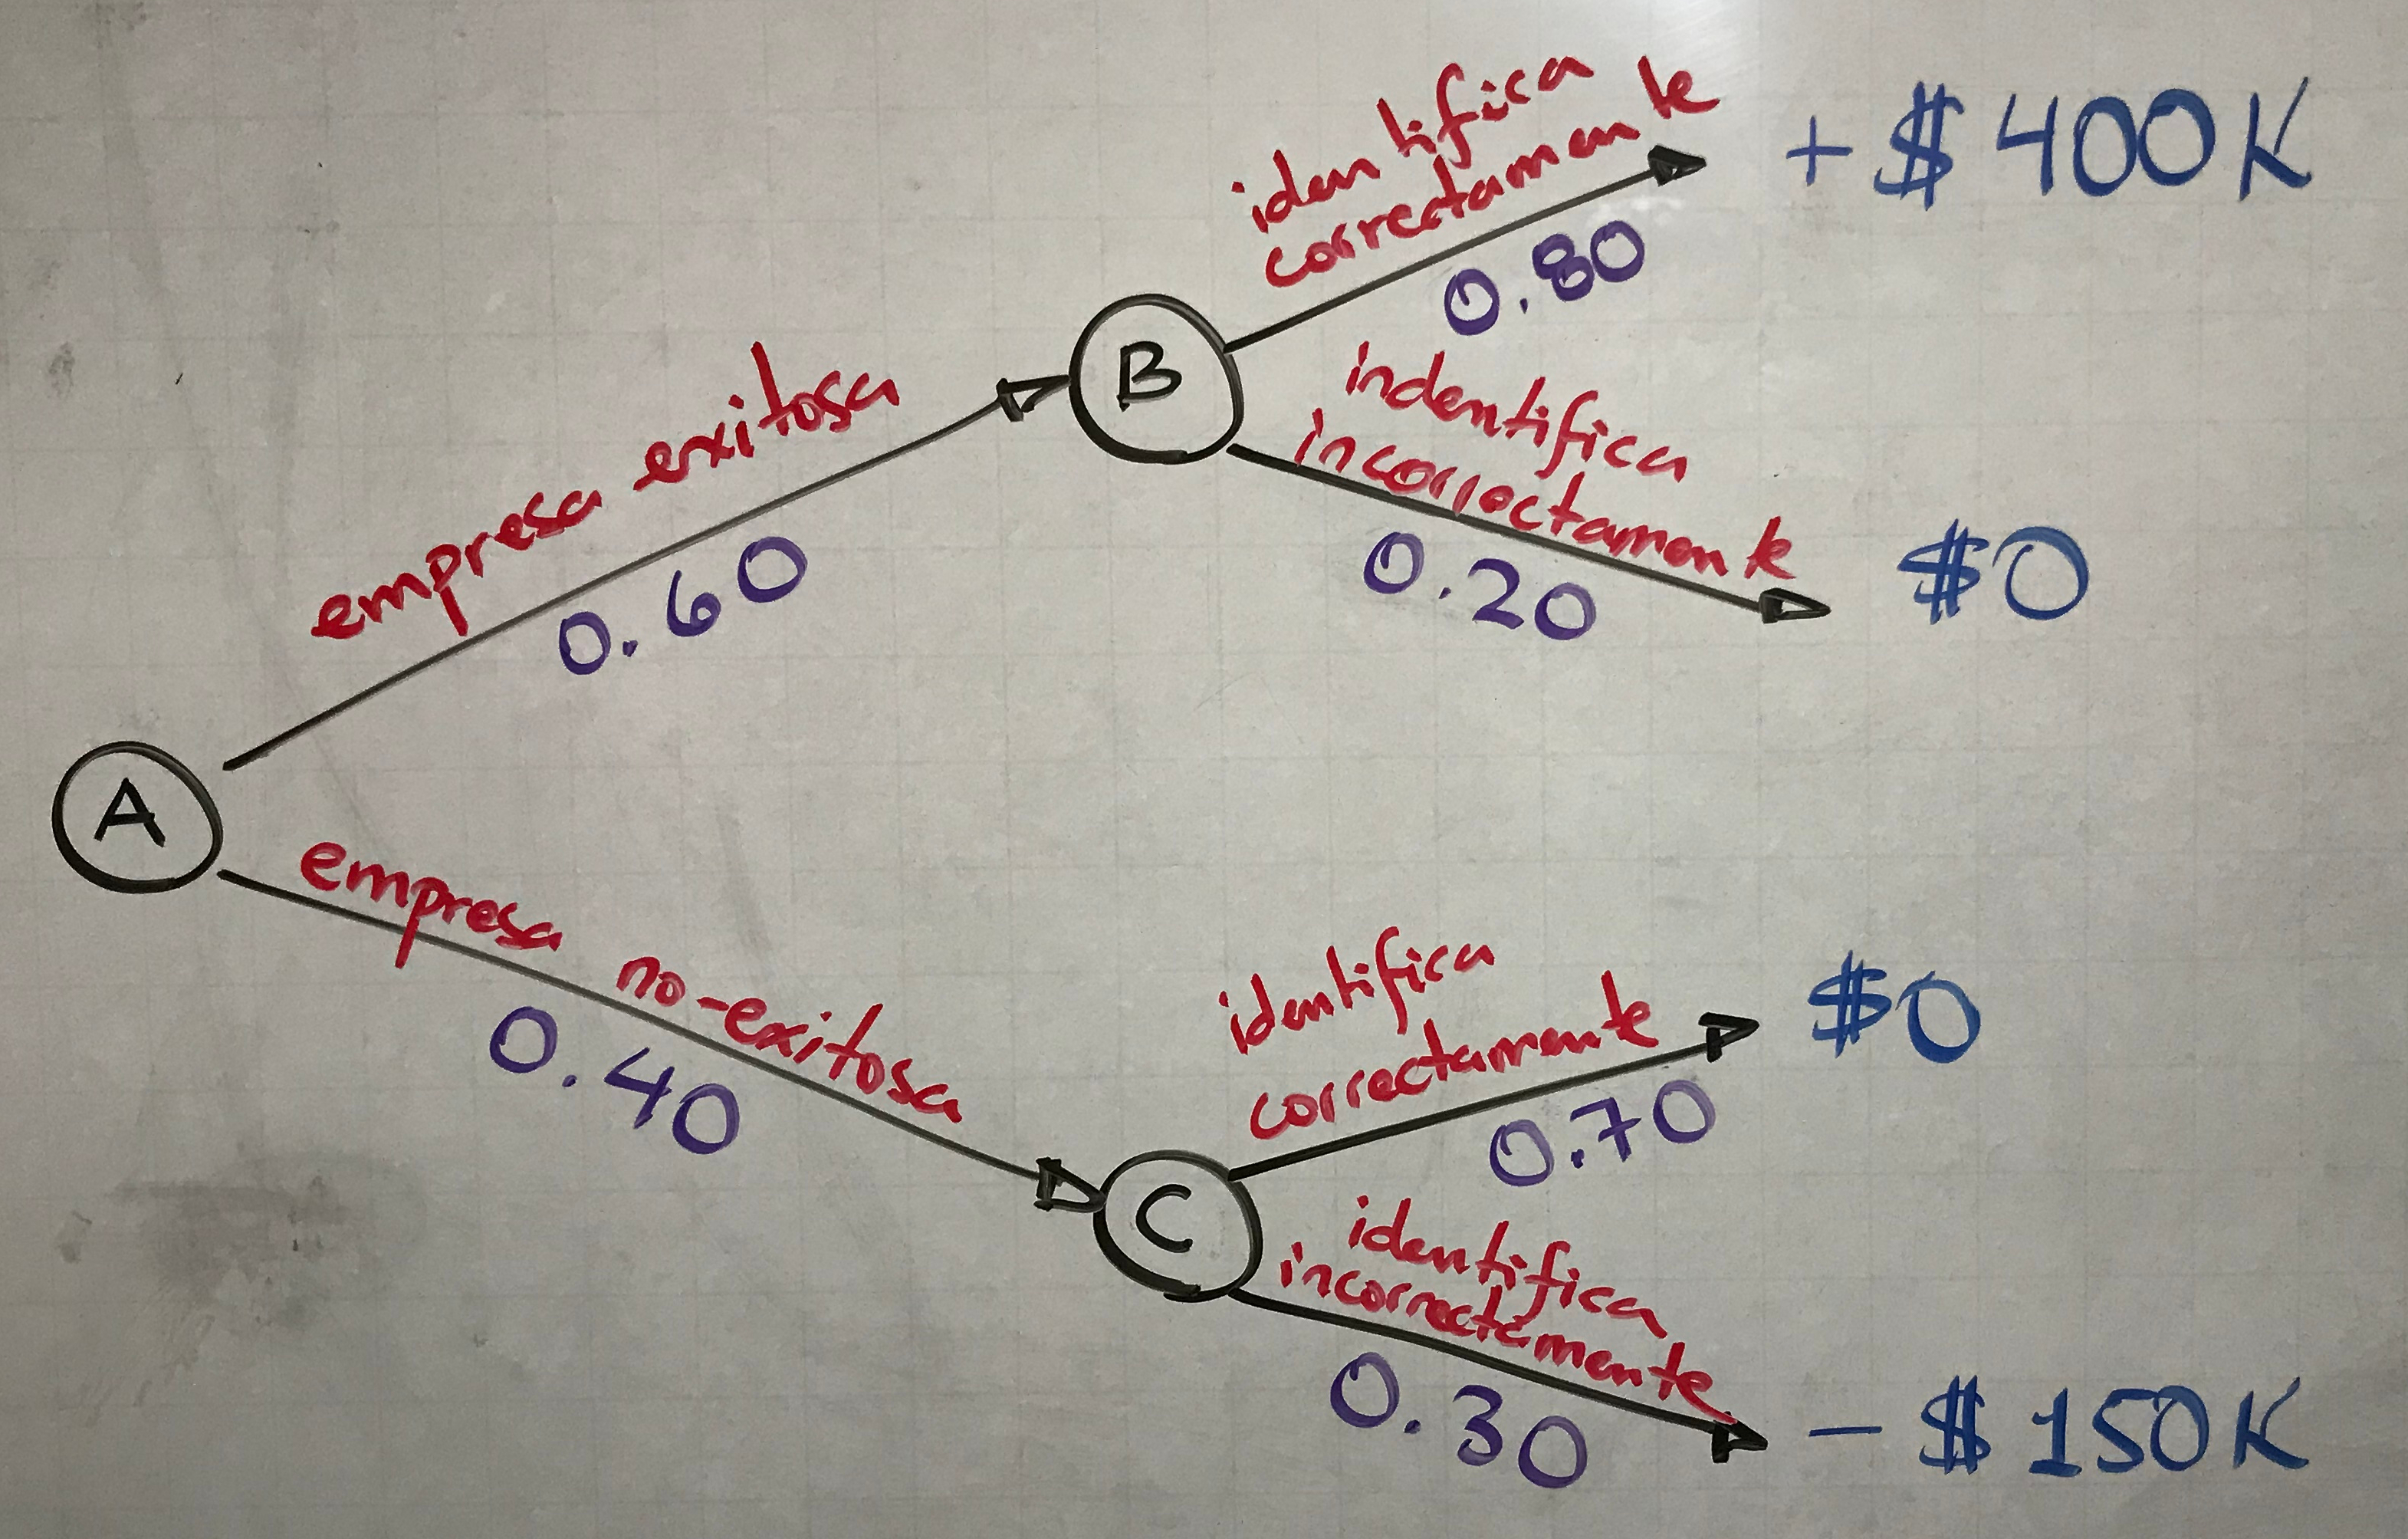
\includegraphics[width=0.66\textwidth]{Problema-3A1.jpg}
\end{figure}
Ahora podamos el \'arbol, calculando la utilidad de los nodos $B$ y $C$, para luego calcular la utilidad del nodo $A$. 
\begin{align*}
\Exp[B] \; 
& = \; (+\$400K)(0.80) + (\$0)(0.20) \; = \; +\$320K \\
\Exp[C] \; 
& = \; (\$0)(0.70) + (-\$150K)(0.30) \; = \; -\$45K \\
& \Longrightarrow \; \Exp[A] \; = \;
(+\$320K)(0.60) + (-\$45K)(0.40) \; = \; +\$174K
\end{align*}

Luego suponemos que el inversionista contrata al consultor. Entonces su \'arbol de probabilidad luce como el que se muestra en la siguiente fotograf\'ia. 
\begin{figure}[H]
\centering
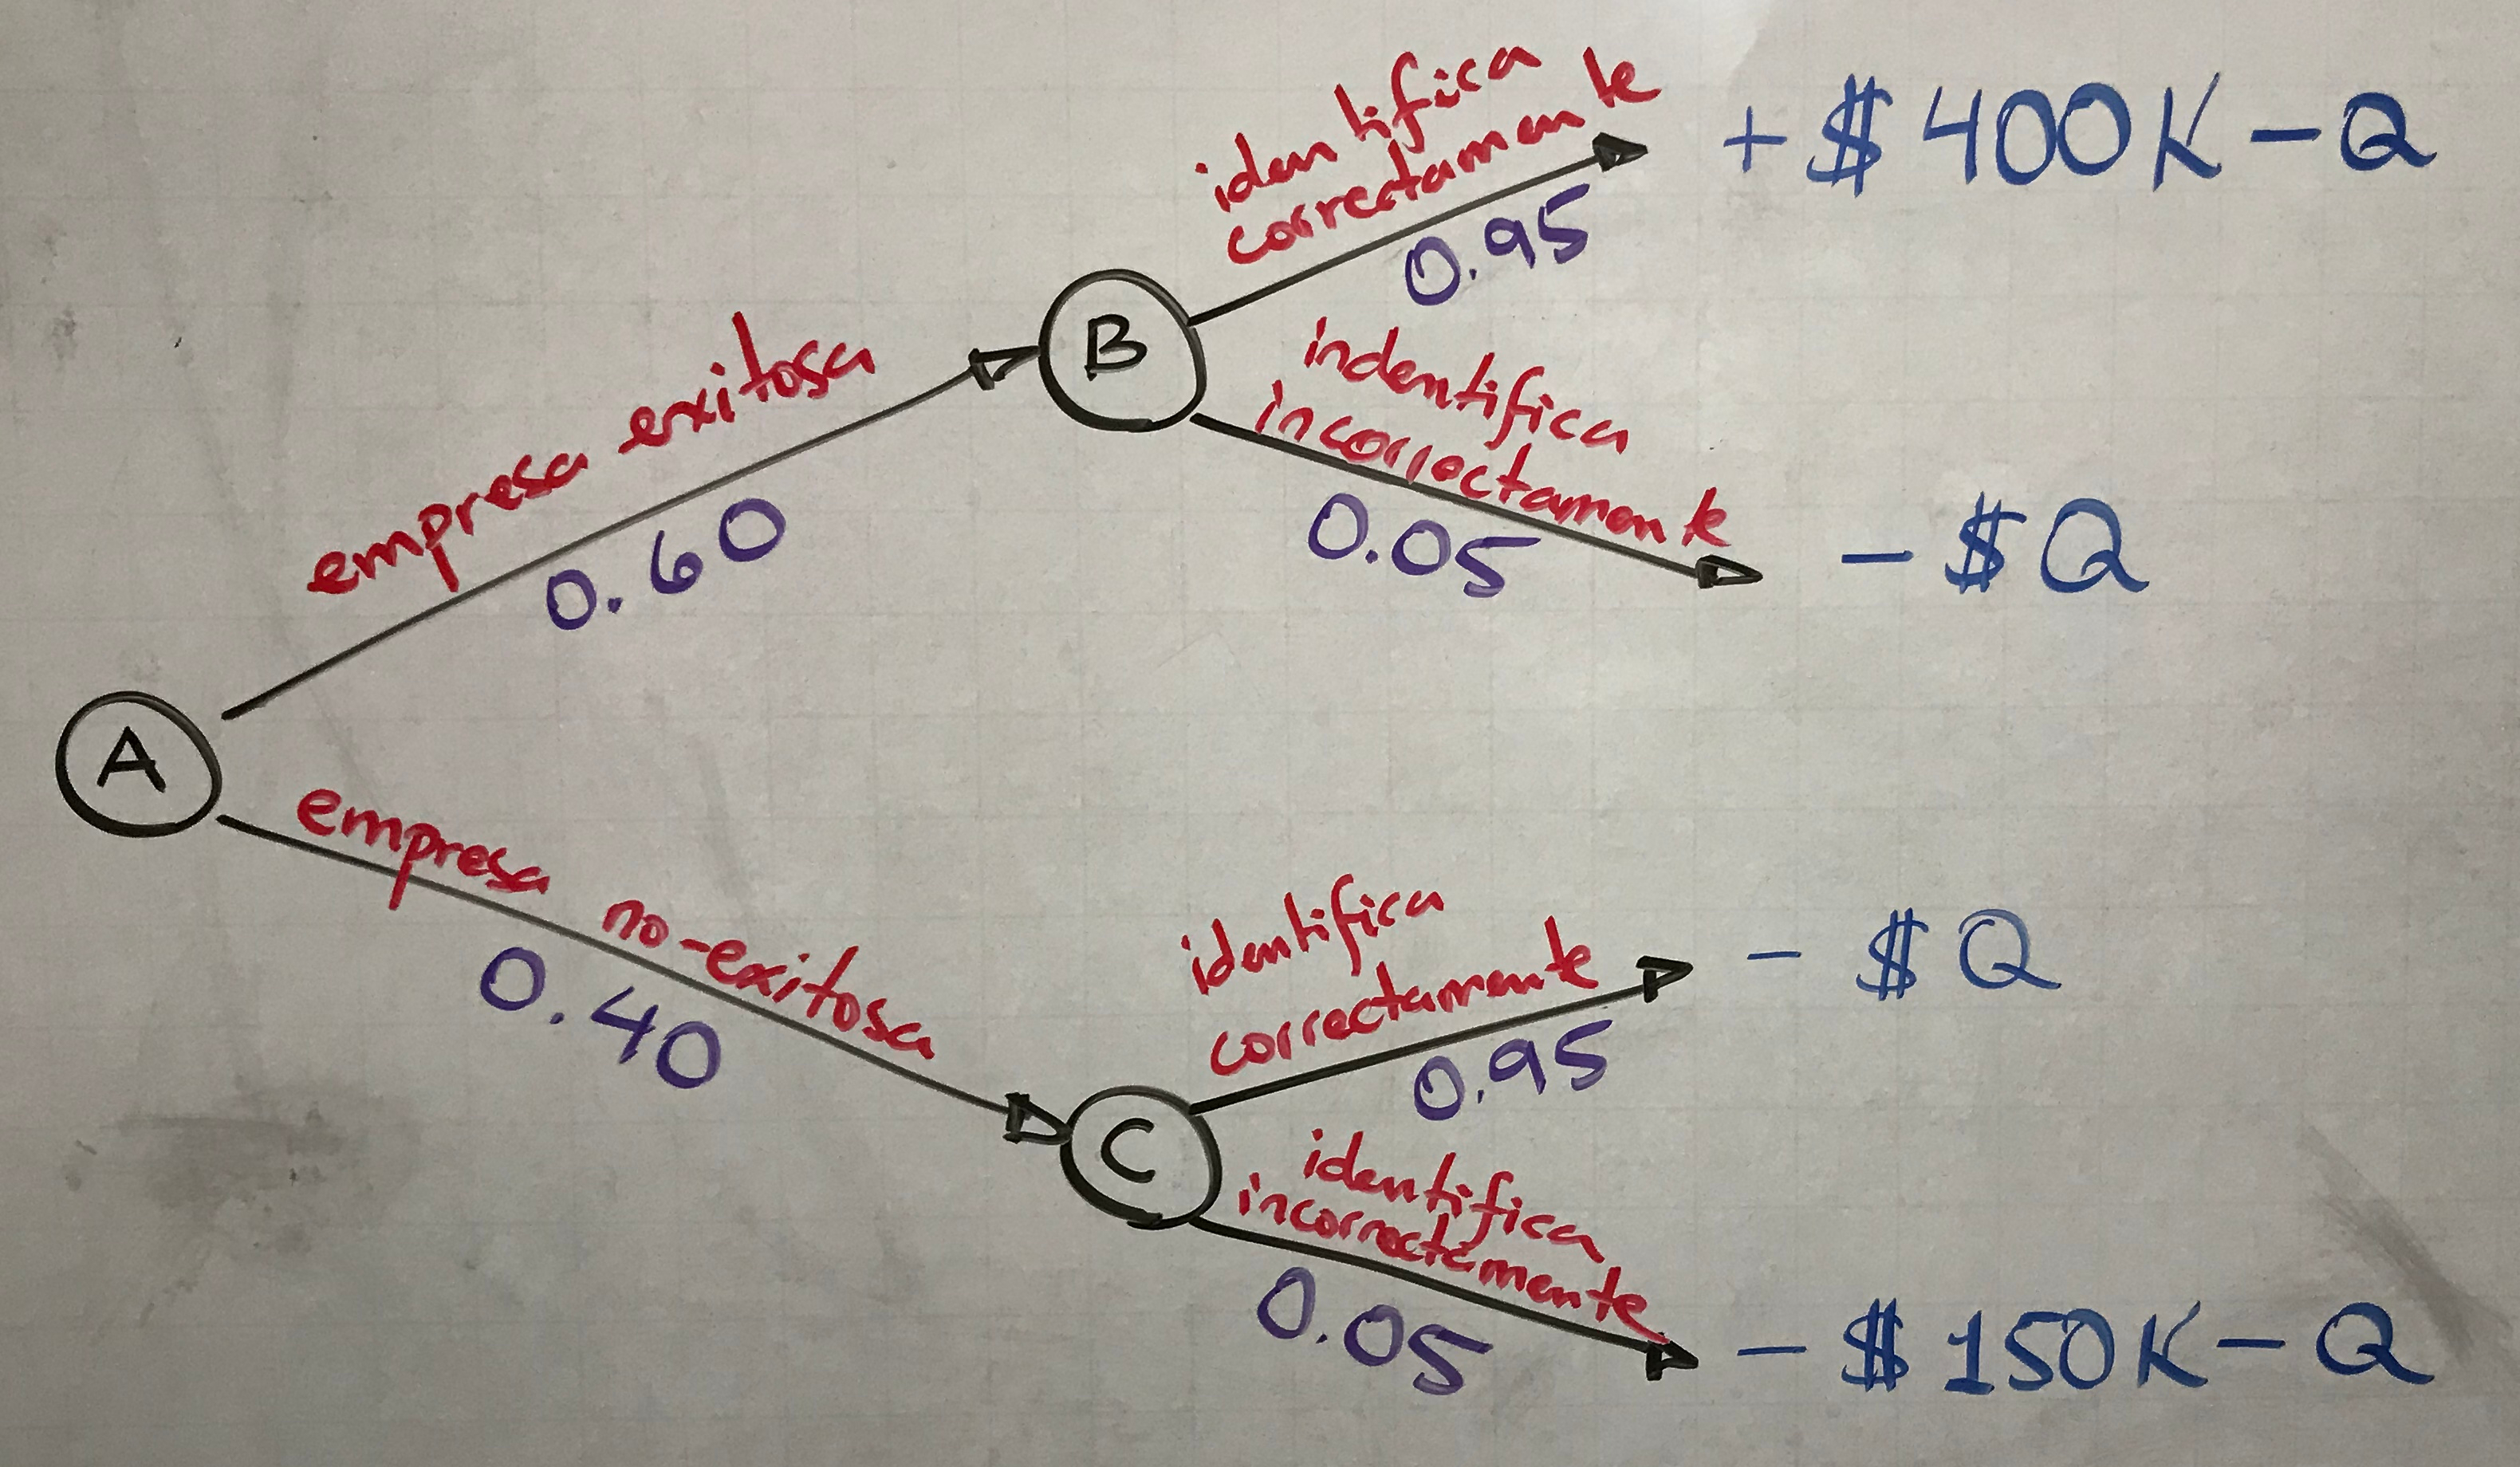
\includegraphics[width=0.66\textwidth]{Problema-3A2.jpg}
\end{figure}
Ahora podamos el \'arbol, calculando la utilidad de los nodos $B$ y $C$, para luego calcular la utilidad del nodo $A$. 
\begin{align*}
\Exp[B] \; 
& = \; (+\$400K-Q)(0.95) + (-\$Q)(0.05) \; = \; +\$380K - Q \\
\Exp[C] \; 
& = \; (-\$Q)(0.95) + (-\$150K - Q)(0.05) \; = \; -\$7.5K - Q \\
& \Longrightarrow \; \Exp[A] \; = \;
(+\$380K - Q)(0.60) + (-\$7.5K - Q)(0.40) \; = \; +\$225K - Q
\end{align*}

Con estos estimados a la mano, vemos que el inversionista contratar\'a al consultor si: 
\[
\$225K - Q \; \geq \; \$174K \quad \Longrightarrow \quad
Q \; \leq \; \$51K
\]
Es conclusi\'on, el m\'aximo honorario que puede cobrar el consultor es de \$51K. 
\QED

\emph{Soluci\'on B:} Primero supongamos que el inversionista no contrata al consultor. Entonces su \'arbol de probabilidad luce como el que se muestra en la siguiente fotograf\'ia. 
\begin{figure}[H]
\centering
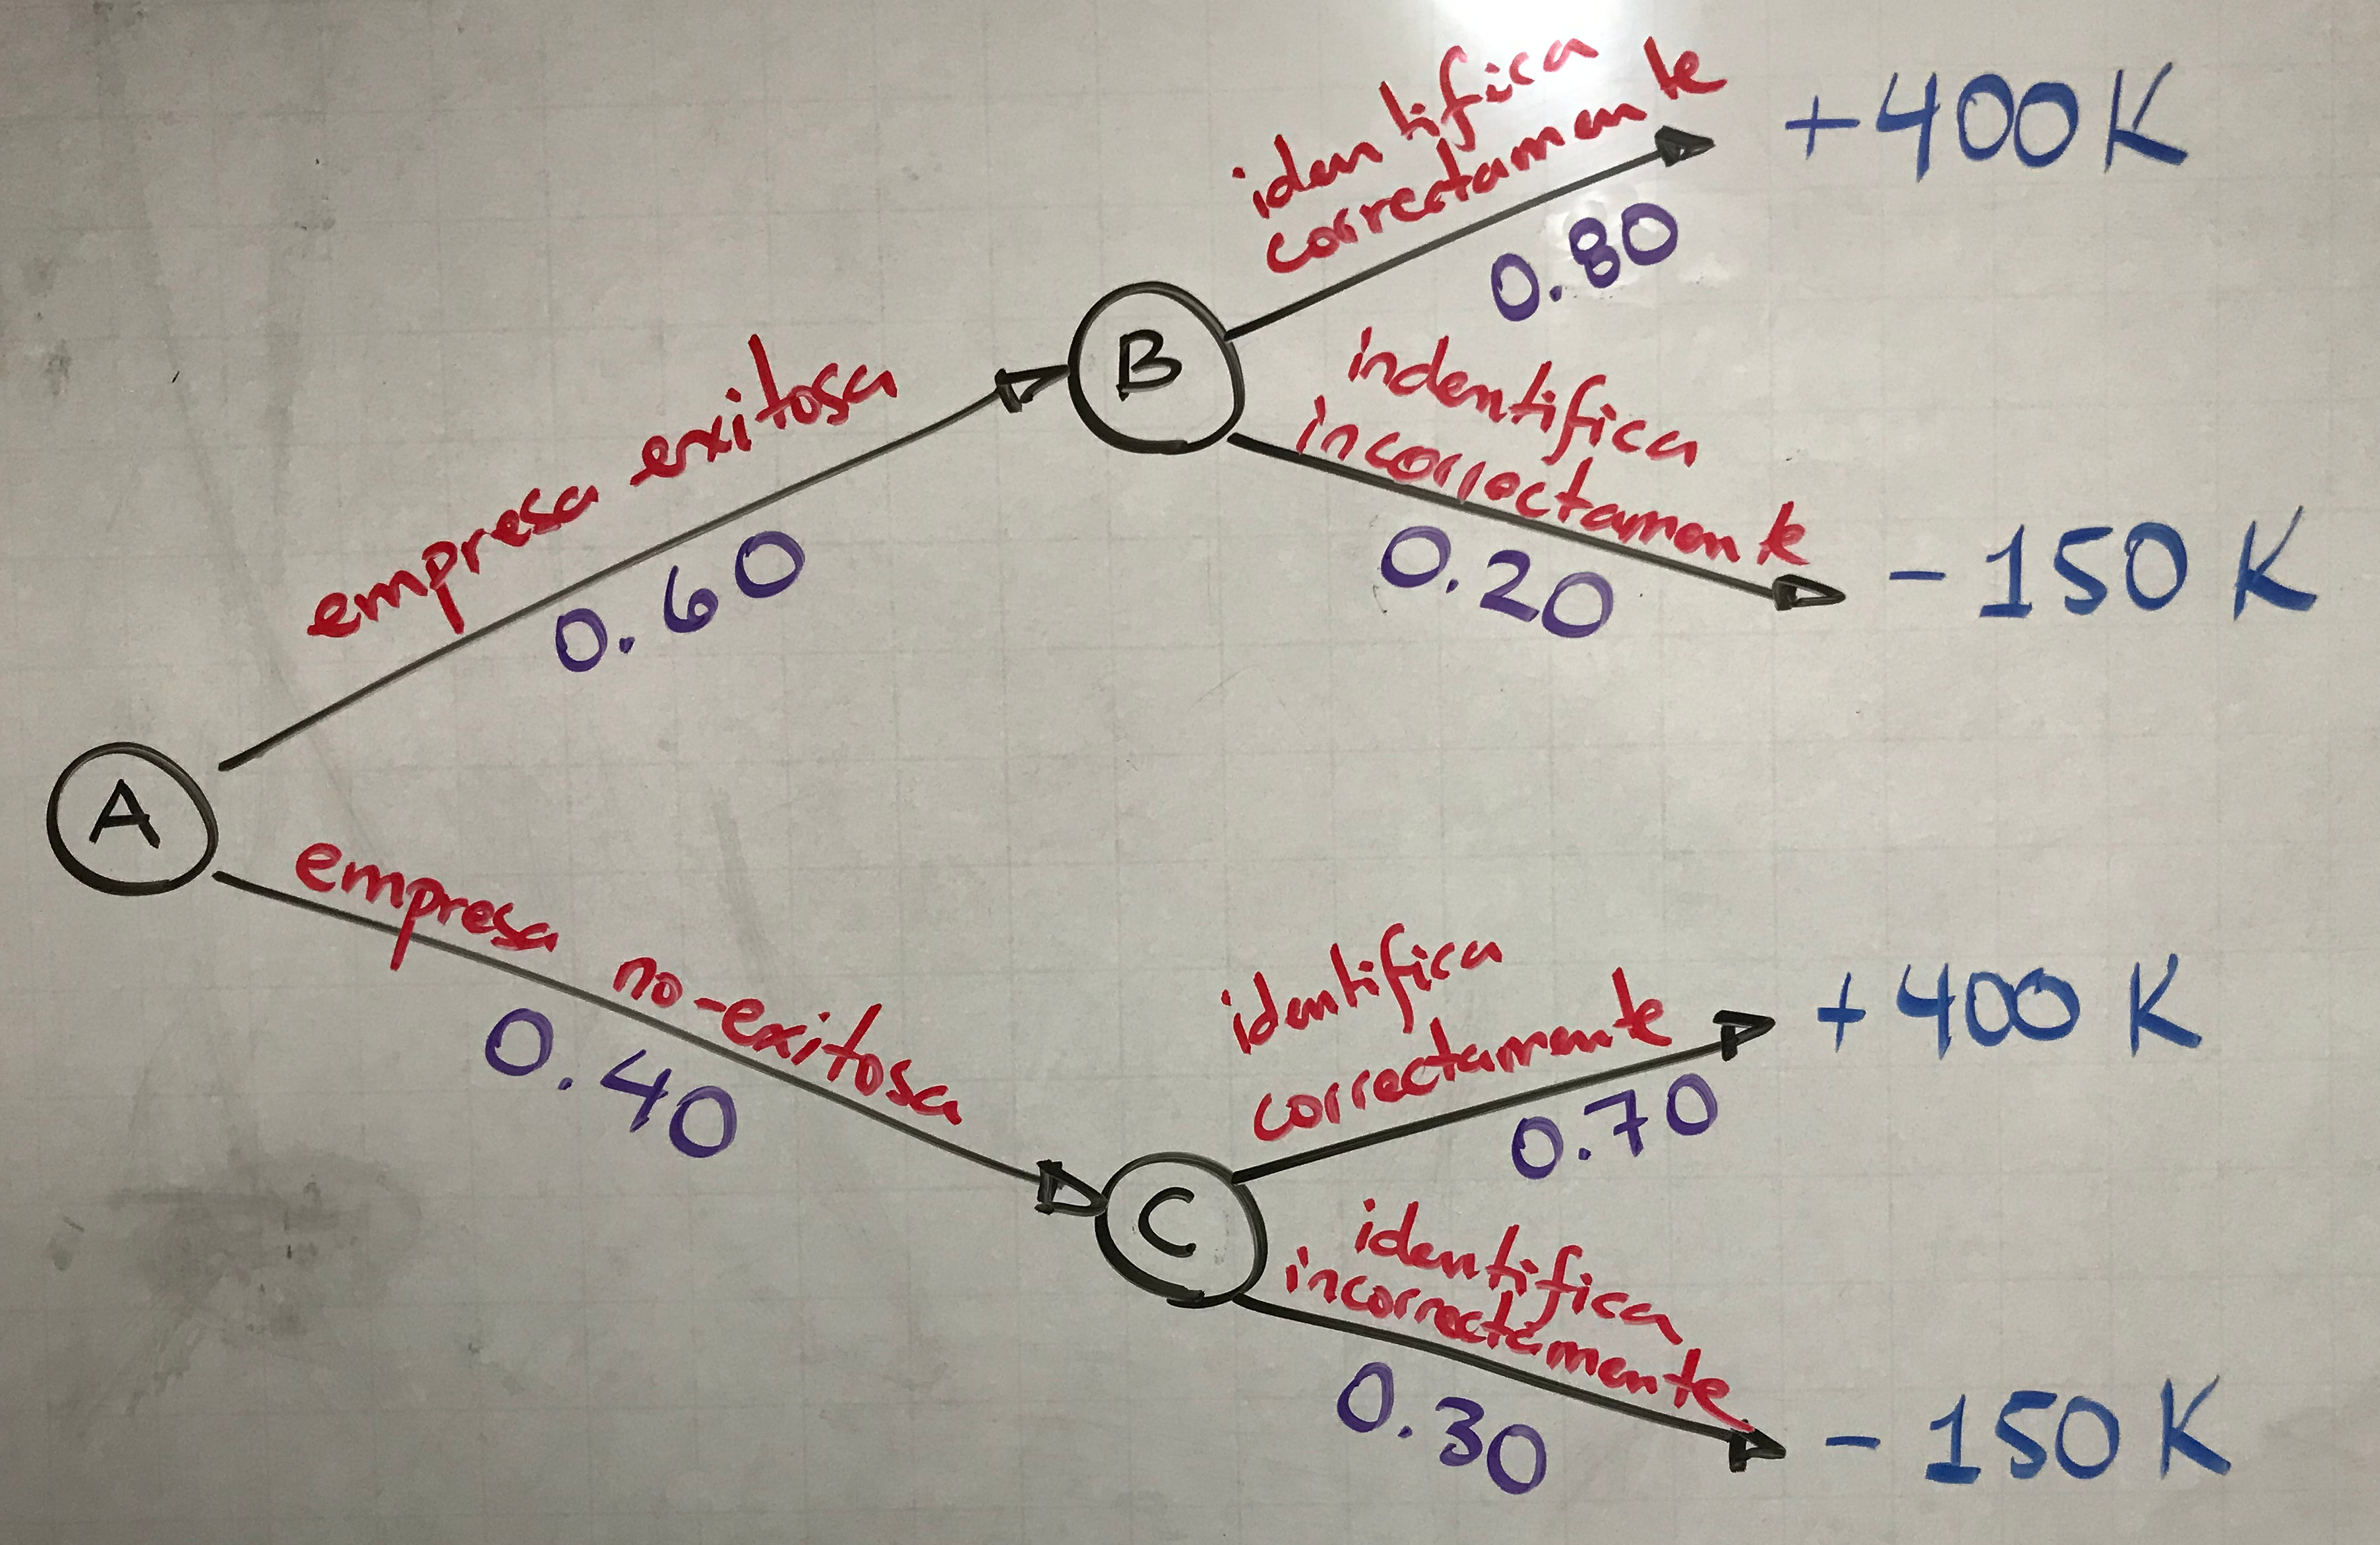
\includegraphics[width=0.66\textwidth]{Problema-3B1.jpg}
\end{figure}
Ahora podamos el \'arbol, calculando la utilidad de los nodos $B$ y $C$, para luego calcular la utilidad del nodo $A$. 

\begin{align*}
\Exp[B] \; 
& = \; (+\$400K)(0.80) + (-\$150K)(0.20) \; = \; +\$290K \\
\Exp[C] \; 
& = \; (+\$400K)(0.70) + (-\$150K)(0.30) \; = \; +\$235K \\
& \Longrightarrow \; \Exp[A] \; = \;
(+\$290K)(0.60) + (+\$235K)(0.40) \; = \; +\$268K
\end{align*}

Luego suponemos que el inversionista contrata al consultor. Entonces su \'arbol de probabilidad luce como el que se muestra en la siguiente fotograf\'ia. 
\begin{figure}[H]
\centering
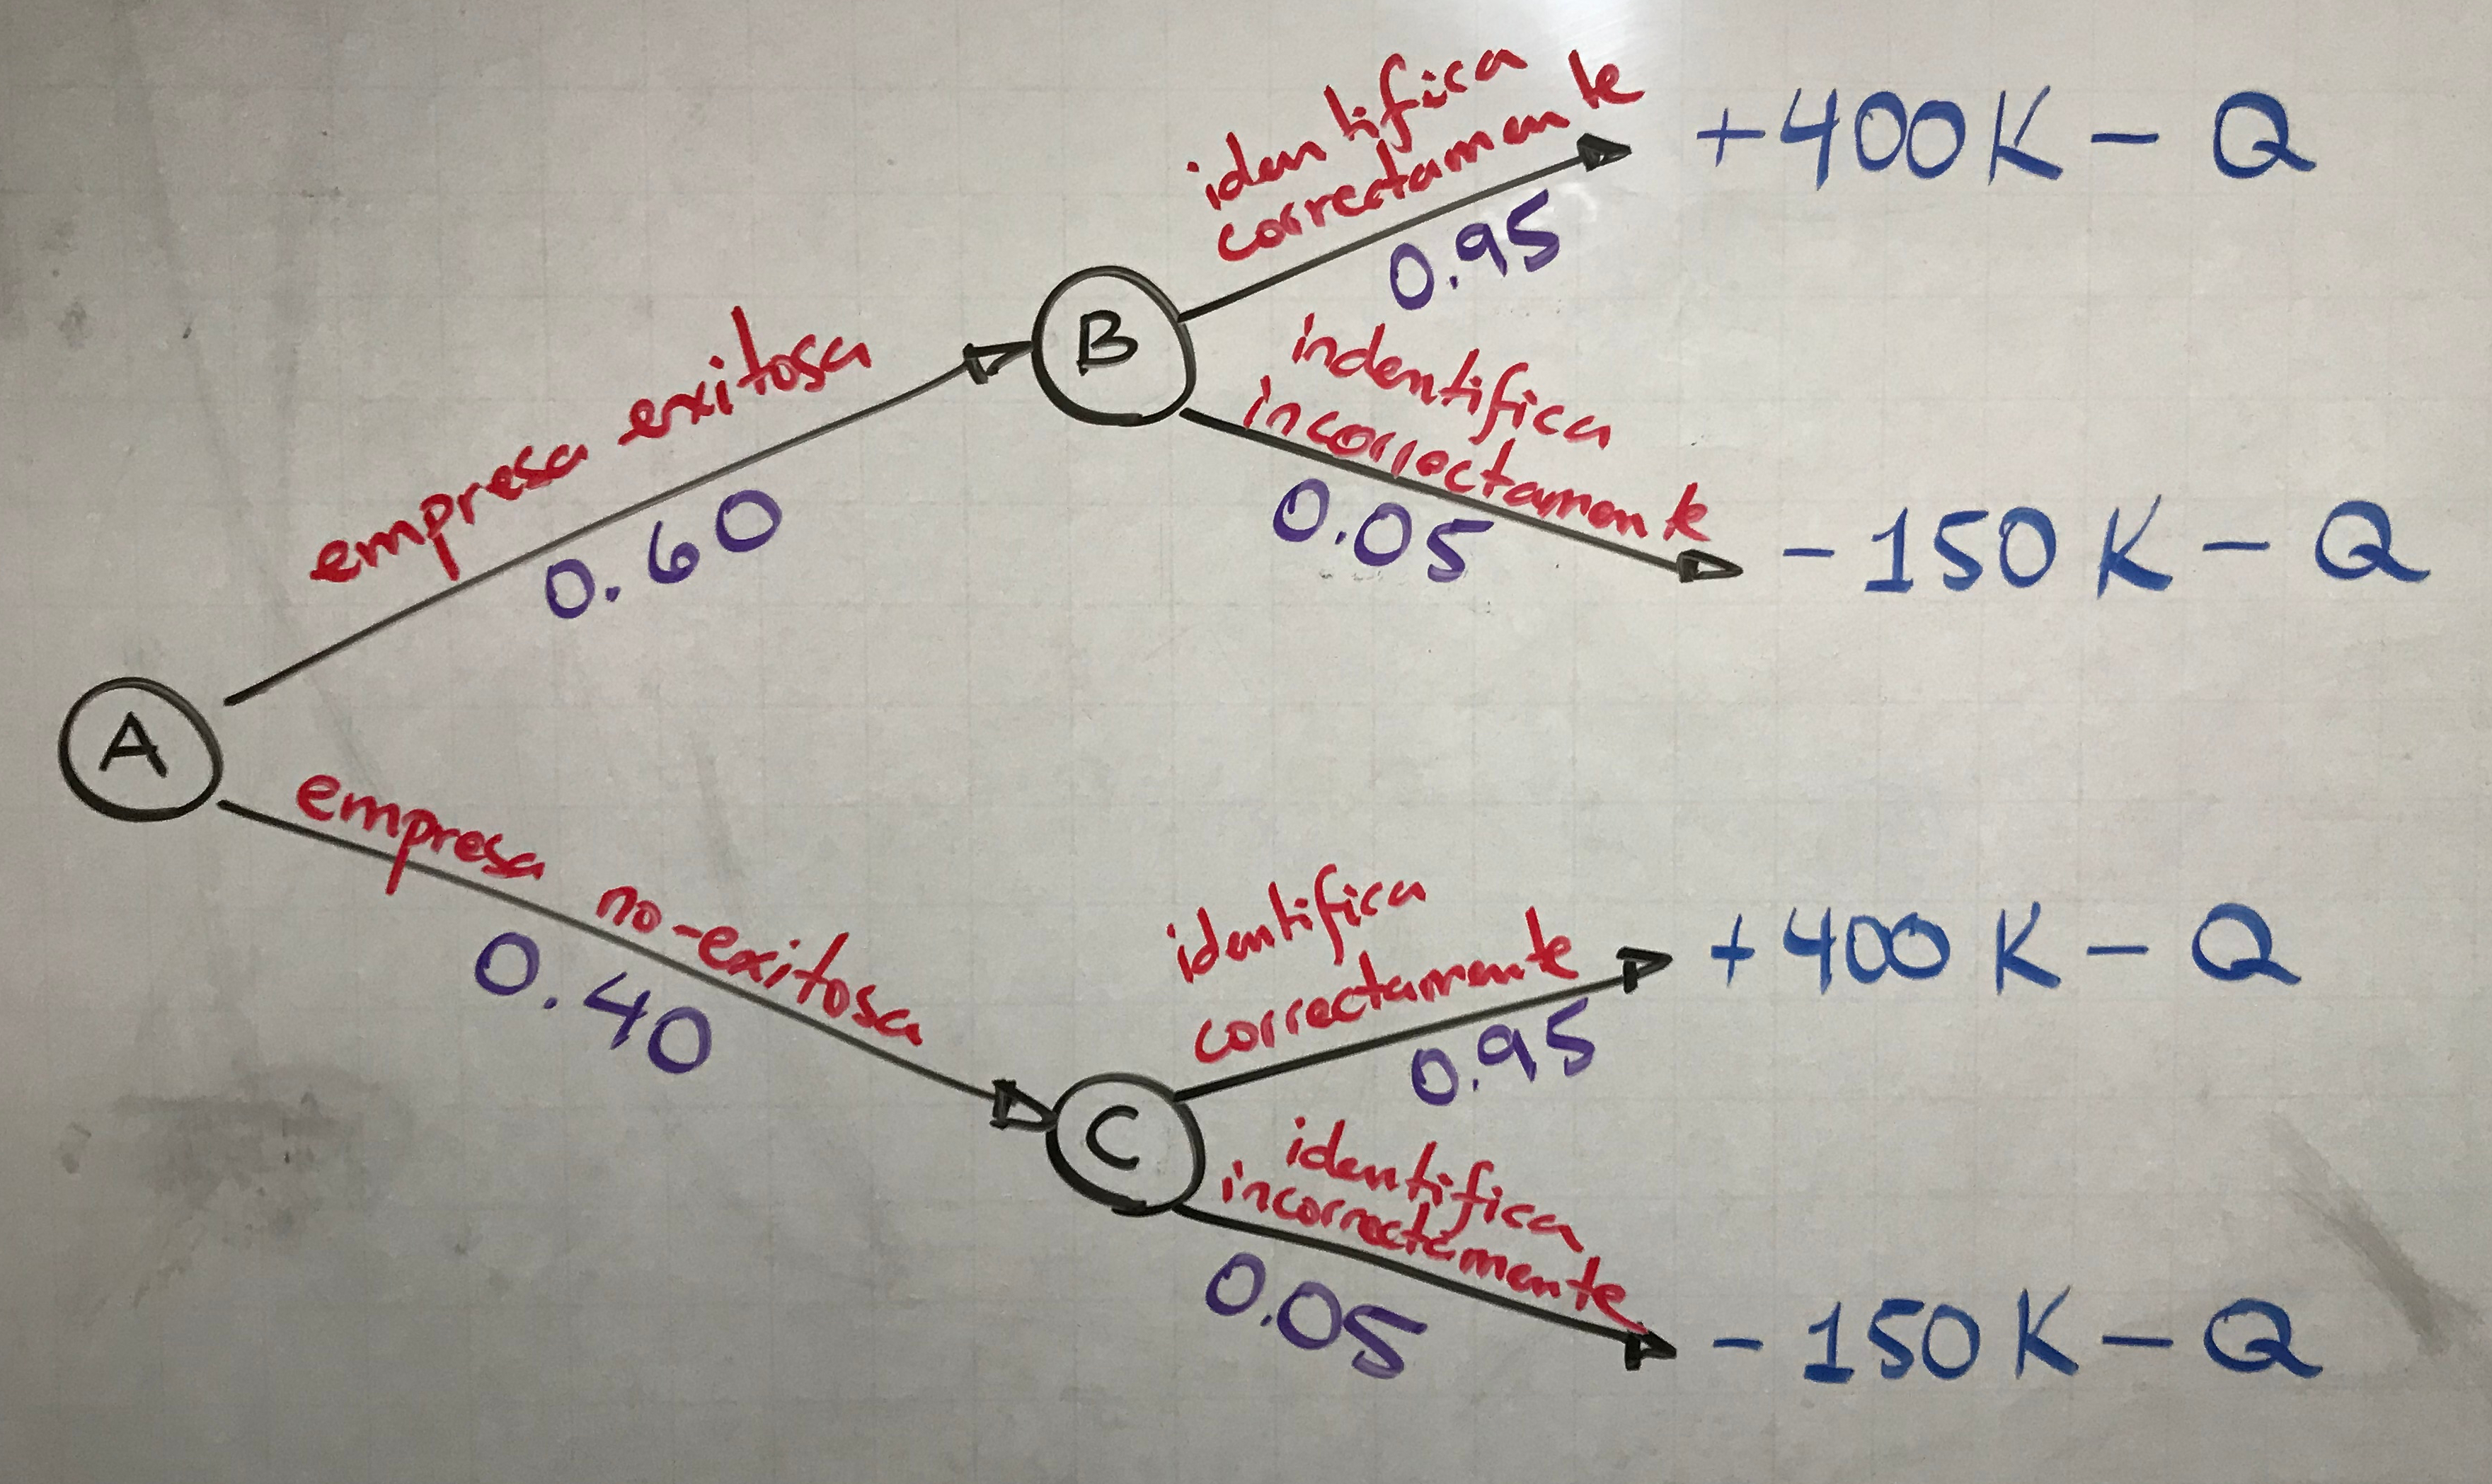
\includegraphics[width=0.66\textwidth]{Problema-3B2.jpg}
\end{figure}
Ahora podamos el \'arbol, calculando la utilidad de los nodos $B$ y $C$, para luego calcular la utilidad del nodo $A$. 
\begin{align*}
\Exp[B] \; 
& = \; \Exp[C] \; = \; (+\$400K-Q)(0.95) + (-\$150K-Q)(0.05) \; = \; +\$372.5K - Q \\
& \Longrightarrow \; \Exp[A] \; = \;
(+\$372.5K - Q)(0.60) + (+\$372.5K - Q)(0.40) \; = \; +\$372.5K - Q
\end{align*}

Con estos estimados a la mano, vemos que el inversionista contratar\'a al consultor si: 
\[
\$372.5K - Q \; \geq \; \$268K \quad \Longrightarrow \quad
Q \; \leq \; \$104.5K
\]
Es conclusi\'on, el m\'aximo honorario que puede cobrar el consultor es de \$104.5K. 
\QED

\end{problem}
\fullskip

\end{document}
